\documentclass{article}
\usepackage{amsmath}
\usepackage{mathtools}
\usepackage{gensymb}
\usepackage[a4paper,inner=1.5cm,outer=1.5cm,top=2cm,bottom=0.5cm]{geometry} 
\usepackage{xcolor}                    
\usepackage{tikz}                           
\usepackage{multicol}
\usepackage{pgfplots}
\usetikzlibrary{calc}
\usetikzlibrary{intersections}
\usetikzlibrary{intersections,calc,angles,quotes}
\usetikzlibrary{shapes,arrows,positioning,decorations.pathreplacing,calc}
\usetikzlibrary{calc,angles,positioning,intersections,quotes,decorations.markings}
\usepackage{tkz-euclide}
\usetikzlibrary{backgrounds}
\usetikzlibrary{calc,through}
\usetikzlibrary{angles}
\usetikzlibrary{fadings}
\usetikzlibrary{shapes.geometric}
\usetikzlibrary{shapes.symbols}
\usepackage{draftwatermark}
\usepackage{mathptmx}

\SetWatermarkText{\textcolor{black!30}{Mathema Shukur}}
\SetWatermarkFontSize{2 cm}
\usepackage[utf8]{inputenc}
\usepackage{fontspec}

\setmainfont{[Kalpurush.ttf]}
\newfontface{\en}{[Arial.ttf]} %%this is optional, if you want to use a secondary font. Any english font is supported
\newlength\Radius
\setlength\Radius{4cm}
\begin{document} 
	\Large
	\textcolor{red}{Welcome To} 
	\\
	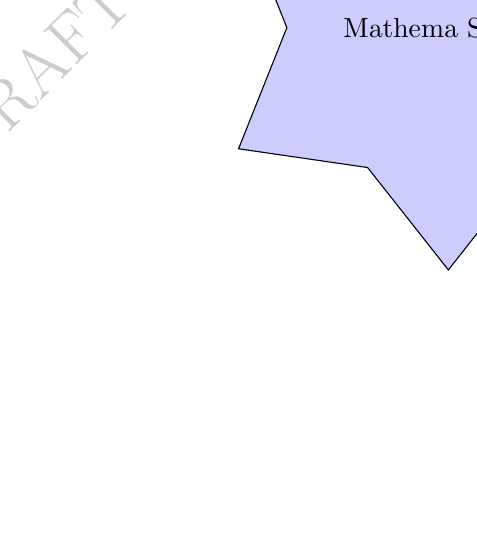
\begin{tikzpicture}
		\tikz \node [fill=blue!20,star,star points=6,draw] {Mathema Shukur };
	\end{tikzpicture}
	\\
	যাদের জন্যে প্রযোজ্যঃ  	\textcolor{magenta}{একাদশ ও দ্বাদশ শ্রেণীর শিক্ষার্থী} \\
	বিষয়ঃ \textcolor{magenta}{উচ্চতর গণিত ১ম পত্র} \\
	অধ্যায়ঃ \textcolor{magenta}{৩-সরলরেখা}\\ 
	Subtopicঃ  \textcolor{magenta}{  সরলরেখার বিভিন্ন আকারের সমীকরণ নির্ণয় করা   }\\
	\\
	\textcolor{blue}{(1)	ঢাল বিন্দু আকার Point slope form}\\
	\\
	$(y-y_1)=m(x-x_1)$\\
	\\
	\textcolor{red} {(2)  দুই বিন্দু আকার 	Two point form}\\
	\\
	$y-y_1=\left(\frac{y_1-y_2}{x_1-x_2}\right)(x-x_1)$\\
	\\
	\textcolor{green}{ (3) ঢাল খণ্ডন আকার 	Slope intercept form}\\
	\\
	$y=mx+c$\\
	\\
	\textcolor{cyan}{ (4) দ্বি খণ্ডন আকার  Two	Intercept form}\\
	\\
	$\frac{x}{a}+\frac{y}{b}=1$\\
	\\
	\vspace{6cm}
	\\
\textcolor{green}{ (3) ঢাল খণ্ডন আকার 	Slope intercept form}\\
\\
$y=mx+c$\\
\\
ঢাল $=m$,\qquad $y-$ অক্ষের খণ্ডিত অংশ $=c$\\
\\ 
	কুমিল্লা বোর্ড-২০২১\\
  একটি সরলরেখার ঢাল $\frac{2}{3}$ এবং $y-$ অক্ষের খণ্ডিত অংশ $-5$ হলে রেখাটির সমীকরণ নির্ণয় কর\\ 
  \\
  $m=\frac{2}{3}$,\qquad $c=-5$\\
  \\ 
  \begin{align*}
  y&=mx+c\\
  \\
  y&=\left(\frac{2}{3}\right)x+(-5)\\
  \\
  3y&=2x-15\\
  \\
  2x-3y-15&=0
  \end{align*}
	\\
\begin{tikzpicture}[transform shape,scale=1]
	\draw [-latex,thick](-3,0) -- (12,0) node[right] {$x$} coordinate(x axis);
	\draw [-latex,thick](0,-7) -- (0,3) node[above] {$y$} coordinate(y axis);
	\fill[black] (0,0) circle (1 mm);
	\node at (0.3,-0.3) {$\textcolor{purple}{O}$};	
	\node at (-0.8,-2) {$\textcolor{cyan}{-5}$};	
	\draw[very thick,magenta] (-3,-7)--(12,3);	
	\draw [cyan,very thick,decorate,decoration={brace,amplitude=12pt,mirror,raise=1ex}]
	(0,0) -- (0,-5);
\end{tikzpicture}
\\
	বরিশাল বোর্ড-২০২১\\ 
$3x+4y-12=0$ সরলরেখাটির ঢাল নির্ণয় কর এবং $y-$ অক্ষ হতে খণ্ডিত অংশের মান নির্ণয় কর \\
\\ 
\begin{align*}
3x+4y-12&=0\\
\\
4y&=-3x+12\\
\\
y&=\frac{-3}{4}x+\frac{12}{4}\\
\\
y&=\frac{-3}{4}x+3\\
&\boxed{\textcolor{blue}{y=mx+c}}\\
\\
m=\frac{-3}{4},&\qquad c=3
\end{align*}
\\
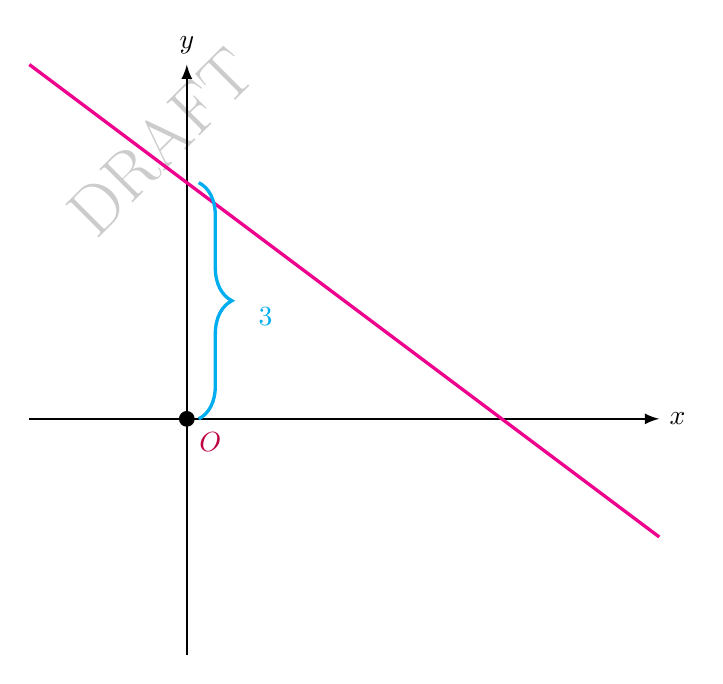
\begin{tikzpicture}[transform shape,scale=1]
	\draw [-latex,thick](-2,0) -- (6,0) node[right] {$x$} coordinate(x axis);
	\draw [-latex,thick](0,-3) -- (0,4.5) node[above] {$y$} coordinate(y axis);
	\fill[black] (0,0) circle (1 mm);
	\node at (0.3,-0.3) {$\textcolor{purple}{O}$};	
	\node at (1,1.3) {$\textcolor{cyan}{3}$};	
	\draw[very thick,magenta] (-2,4.5)--(6,-1.5);	
	\draw [cyan,very thick,decorate,decoration={brace,amplitude=12pt,mirror,raise=1ex}]
	(0,0) -- (0,3);
\end{tikzpicture}
\end{document}